\section{Hierarchie výpočetní složitosti. Třídy složitosti P, NP, \#P, PSPACE, EXP, NP-těžké. Definice problému Problém batohu (Knapsnack), problém směrování vozidel (VRP), Metrický k-střed.}

\subsection{Polynomická vs exponenciální časová složitost.}

Algoritmy s~polynomickou složitostí lze efektivně řešit, bez vynaložení velkého výpočetního výkonu. 
S délkou vstupu \textit{n} roste lineárně potřebný čas ($n^x$) například hledání nejkratší cesty. 
Algoritmy s~exponenciální složitostí lze efektivně řešit pouze pro malé exponenty, bez potřeby velkého výpočetního výkonu. 
S délkou vstupu \textit{n} roste exponenciálně potřebný čas ($x^n$) například problém obchodního cestujícího.

\subsection{Hierarchie výpočetní složitosti.}

Hierarchie výpočetní složitosti slouží k~charakterizaci algoritmů u kterých lze pouze nepřímo určit asymptotickou složitost. 
Využívá se třídní hierarchie. 
Třídy od nejjednodušší po nejsložitější jdou v~tomto pořadí: P $\subseteq$ NP $\subseteq$ \#P $\subseteq$ PSPACE $\subseteq$ EXP $\subseteq$ NP-složité $\subseteq$ unsolvable. 
Jednoduší třída je vždy podmnožinou složitější (do složitější patří i ty jednoduší).

\subsection{Třída P}

Třída P obsahuje polynomiální problémy. 
Tyto problémy se dají vyřešit v~polynomiálním čase na~deterministickém Turingově stroji (TS). 
Příkladem může být nalezení nejkratší cesty, minimální kostry v~grafu.

\subsection{Třída NP}

Třída NP obsahuje nedeterministické polynomiální problémy. 
Tyto problémy lze řešit v~polynomiálním čase na~nedeterministickém TS (doposud nesestaven).

\subsection{Třída NP-complete (NP-úplné)}

NP-úplné (NPC) je podskupina problémů třídy NP, která se zabývá rozhodovacími problémy.
Jejich řešení je nejtěžší a všechna známá řešení lze na~deterministickém TS provést pouze s~exponenciálním čase. 
Pro polynomiální nebylo zatím nalezeno řešení, ale zároveň nebylo dokázáno, že řešení neexistuje.

\textbf{Problém NPC}\,--\,pokud by se podařilo, převést jeden NPC problém na~polynomiální čas tak to znamená, že každý NPC problém lze převést do~polynomiálního. 
To by vedlo k~prokázání P $=$ NP.

Bylo dokázáno, že každý algoritmus pro NPC problém lze použít k~řešení jiného NPC problému.
Přibližně existuje 10\,000 známých NPC problémů.
Příkladem může být\,--\,Barvení grafů, Knapsnack (problém batohu), 3-partition problém (rozdělit množinu čísel podmnožiny o velikosti 3, které mají stejný součet)

\subsection{Třída NP-těžké}

O problému řekneme, že je NP-težký, jestliže se na~něj redukuje NPC problém, ale zároveň nevíme jestli spadá do~NP.
Redukce znamená že se dá převést/konvertovat.

\subsection{P vs NP}

P je podmnožina NP jelikož každý problém lze řešit v~polynomiálním čase na
 nedeterministickém TS.
Existuje matematický problém P $=$ NP, který dosud nebyl potvrzen nebo vyvrácen. Takže se přesně nedá určit jestli je P $=$ NP. 
Obecně se považuje, že P $\neq$ NP.

\subsection{Třída \#P}

Třída \#P se nezabývá rozhodovacími problémy, ale řeší problém nalezení možných řešení NP problémů. 
Z toho plyne, že problémy třídy \#P musí být alespoň stejně složité jako stejný NP problém.
U této třídy se neptáme jestli existuje řešení, ale kolik řešení existuje.

\textbf{Definice:} \#P je množina všech funkcí $f(x)$, kde $f(x)$ odpovídá počtu přijatelných cest nedeterministického TS v~polynomiálním čase.

\noindent V této třídě existují také problémy \#P-úplné.

\subsection{Třída PSPACE}

PSPACE je množina rozhodovacích problémů, které lze vyřešit pomocí deterministického TS v~polynomiálním paměťovém prostoru.
Neboli nezáleží, jak dlouho trvá vykonání, když je využit polynomiální (rozumné) množství paměťi. 
PSPACE má úplné problémy, které jsou sestupně samo redukovatelné (downward self-reducible) a náhodně samo redukovatelné (random self-reducible).
Jsou zahrnuté v~EXP.
Dle Savitchova theorému můžeme dokázat, že \textbf{P}SPACE = \textbf{NP}SPACE.

\subsection{Třída EXP}

Často označována jako EXPTIME.
Je to množina rozhodovacích problémů řešitelných na~deterministickém TS v~exponenciálním čase.
Časová komplexita je O($2^{p(n)}$), kde $p(n)$ je polynomická funkce $n$.

Existuje také třída EXPSPACE, která je podobná EXPTIME, jen se neřeší v~exponenciálním času, ale v~exponenciálním paměťovém prostoru.

U obou tříd se jedná o nezvládnutelné problémy, pro které neexistuje polynomiální algoritmus.
Jejich složitost je exponenciální (například $2^n$).

\subsection{Knapsnack problém}

Existuje osoba (zloděj), který má batoh/zavazadlo.
Zavazadlo má určitou maximální hmotnost/velikost.
Zloděj se snaží do~batohu vložit co nejvíce zboží v~co největší hodnotě. 
Každé toto zboží má jinou hmotnost/velikost a jinou hodnotu.
Takže zloděj hledá co nejoptimálnější zboží, které může vložit do~batohu a tím mít co největší profit.

\subsection{Problém směrování vozidel (VRP)}

Existuje 1 místo (sklad), která má x vozidel.
Vozidla ze skladu musí objet všechny místa a dovést tam zboží. 
Vozidla nemusí navštívit stejný počet míst, ale množina vozidel musí navštívit všechna místa co nejoptimálněji. 
Při jednom vozidle podobné problému obchodního cestujícího (TSP), jen s~rozdílem, že u TSP si vybíráme začátek, ale u VRP máme začátek přesně definován.

\subsection{Metrický k-střed}

Máme x měst a mezi těmito městy je přesně definována vzdálenost.
Můžeme ale umístit pouze n skladišť, takže skladiště bude obstarávat více měst. 
Do některých měst chceme umístit skladiště, které bude obstarávat dalších x měst.
Musíme vybrat nejvhodnější města pro postavení skladu, aby maximální vzdálenost každého města ke skladu byla co nejmenší.


\clearpage
\section{Problém obchodního cestujícího a modifikace genetických algoritmů, Genetické programování, Optimalizace hejnem, Optimalizace mravenčí kolonií, Evoluční strategie.}

\subsection{Problém obchodního cestujícího}

V~tomto NP-těžkém problému (\emph{Travelling Salesman Problem, TSP}) jde o~nalezení té nejkratší Hamiltonské cesty v~grafu $G$:
Hamiltonská cesta $P$ je taková cesta, která navštíví každý vrchol právě jednou.

Heurestické algoritmy negarantují že nalezly nejlepší řešení, ale operují v~dosažitelném čase.
Příkladem je \href{https://en.wikipedia.org/wiki/Nearest_neighbour_algorithm}{Nearest Neighbour} (dochází k~\enquote{slepému} propojování nejbližších bodů bez~znalosti celku), který může vrátit nejlepší i~nejhorší možný výsledek.

\subsubsection{Modifikace genetických algoritmů pro~TSP}

Genetické algoritmy nejdou na~TSP aplikovat přímo, protože každý z~vrcholů může být navštíven pouze jednou.

\begin{itemize}
\item přirozený výběr: fitness funkce je celková délka cesty a~nevyžaduje modifikaci
\item mutace: prohození dvou vrcholů uvnitř chromozomu nevyžaduje modifikaci
\item křížení: nestačí vyměnit dvě části chromozomu, je třeba ho \enquote{přefiltrovat} a~vybrat pouze takové vrcholy, které se v~chormozomu ještě neobjevily (a~tyto vyfiltrované nahradit)
\end{itemize}

\subsection{Genetické programování}

Genetické programování pracuje se~stromy, ne vektory.
Strom obsahuje pouze funkce a~terminály (které jsou pouze v~listech a nemají potomky).

Náhodně generované programy využívají základní operace a~konstanty pro~rozhodovací strom s~omezenou hloubkou.
Vybraná funkce rekurzivně generuje další stromy.
Ekvivalent křížení je prohození podstromů.

\begin{figure}[ht]
    \centering
    \tikzstyle{node}=[circle, draw, text centered]
    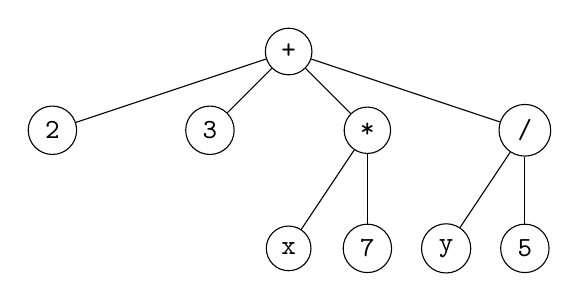
\begin{tikzpicture}
        \node[node](+) at (3, 3) {\texttt{+}};

        \node[node](2) at (0, 2) {\texttt{2}};
        \node[node](3) at (2, 2) {\texttt{3}};
        \node[node](*) at (4, 2) {\texttt{*}};
        \node[node](/) at (6, 2) {\texttt{/}};

        \node[node](x) at (3, 0.5) {\texttt{x}};
        \node[node](7) at (4, 0.5) {\texttt{7}};
        \node[node](y) at (5, 0.5) {\texttt{y}};
        \node[node](5) at (6, 0.5) {\texttt{5}};

        \begin{scope}[every path/.style={-}, every node/.style={inner sep=1pt}]
            \draw (2) -- node {} (+);
            \draw (3) -- node {} (+);
            \draw (*) -- node {} (+);
            \draw (/) -- node {} (+);

            \draw (x) -- node {} (*);
            \draw (7) -- node {} (*);
            \draw (y) -- node {} (/);
            \draw (5) -- node {} (/);
        \end{scope}
    \end{tikzpicture}
    \caption{Strom řešící příklad $5 + 7x + y/5 = 0$}
\end{figure}
\FloatBarrier

\subsection{Optimalizace hejnem}

Každá částice se snaží aktualizovat svou pozici $X$ v~prostoru (2D, 3D, \dots):

$$X(t+1) = X(t) + V(t+1)$$
$$V(t+1) = WV(t) + C_1 \cdot \mathrm{\texttt{rand()}} X (X_\mathrm{pbest} - X(t)) + C_2 \cdot \mathrm{\texttt{rand()}} X (X_\mathrm{gbest} - X(t))$$
%
kde $V(t)$ je rychlost v~čase $t$, $X(t)$ je pozice v~čase $t$, $W$ je váha, $C_1$/$C_2$ jsou učící a~akcelerační faktory, rand je reálné číslo $<0, 1>$, $X_\mathrm{pbest}$ je nejlepší osobní pozice částice a~$X_\mathrm{gbest}$ je globální nejlepší pozice.

Jedna iterace algoritmu, tj. výpočet fitness funkce:

\begin{enumerate}
\item aktualizace osobního i~globálního nejlepšího výsledku,
\item aktualizace rychlosti částic,
\item aktualizace pozice částic.
\end{enumerate}

\subsection{Optimalizace mravenční kolonií}

Simuluje mnoho nezávislých kooperujících jedinců:

\begin{enumerate}
\item vytvoření částečného řešení,
\item přidání hrany na~základě stochastických parametrů a~feromonů,
\item vyhledání lokálního minima,
\item aktualizace feromonů dobrých řešení.
\end{enumerate}

\subsection{Evoluční strategie}

Využívá pouze mutaci, ne křížení.
Jednotlivci jsou většinou reprezentováni jako pár vektorů reálných čísel: $v = (x, \sigma)$, kde $x$ je souřadnice pozice a~$\sigma$ je vektor směrodatných odchylek v~daném bodu.

\clearpage
\section{Definice grafu. Incidenční matice, matice sousednosti. Handshaking lemma. Algoritmus detekce bipartitního grafu. Silně propojené komponenty. Kosarajův algoritmus. Tarjanův algoritmus.}

Graf je matematická struktura $G = (V, E)$: uspořádaná dvojice množin vrcholů a~hran (\emph{vertices and edges}), kde hrana je určena dvěma vrcholy a~volitelně směrem nebo váhou.
Velké množství problémů postavených nad~grafy je NP-úplných.

\subsection{Maticové reprezentace}

Incidenční matice obsahuje informace o~mapování vrcholů jednotlivým hranám.
Matice má řádek pro~každý vrchol a~sloupec pro každou hranu; pokud vrchol hraně náleží, je na~pozici jednička (pro~orientované grafy může mít výchozí vrchol hodnotu $-1$).

Matice souslednosti má podobu čtvercové matice $n \times n$ (kde $n$ je počet vrcholů grafu), jejíž hodnota na~místě $a_{i,j}$ je celé číslo odpovídající počtu hran vedoucích z~vrcholu $i$ do~vrcholu $j$, prvky na~diagonále pak odpovídají počtu hran vedoucích z~vrcholu $i$ do~vrcholu $i$.

Incidenční matice
% TODO Zde by šlo obsah matice obarvit -- pro každou hranu jiná barva.
% TODO Jak se značí když je vrchol propojený sám se sebou? Stačí tam ta jednička?
$\left( \begin{matrix}
1 & 1 & 1 & 0 & 0 & 0 & 0 \\
0 & 1 & 0 & 1 & 0 & 0 & 0 \\
0 & 0 & 0 & 1 & 1 & 0 & 0 \\
0 & 0 & 0 & 0 & 1 & 1 & 1 \\
0 & 0 & 1 & 0 & 0 & 1 & 0 \\
0 & 0 & 0 & 0 & 0 & 0 & 1 \\
\end{matrix} \right)$ 
i matice souslednosti
$\left( \begin{matrix}
2 & 1 & 0 & 0 & 1 & 0 \\
1 & 0 & 1 & 0 & 1 & 0 \\
0 & 1 & 0 & 1 & 0 & 0 \\
0 & 0 & 1 & 0 & 1 & 1 \\
1 & 1 & 0 & 1 & 0 & 0 \\
0 & 0 & 0 & 1 & 0 & 0 \\
\end{matrix} \right)$
popisují vlastnosti grafu na~obrázku \ref{ilustracni-graf-matice}.

\begin{figure}[ht]
\centering
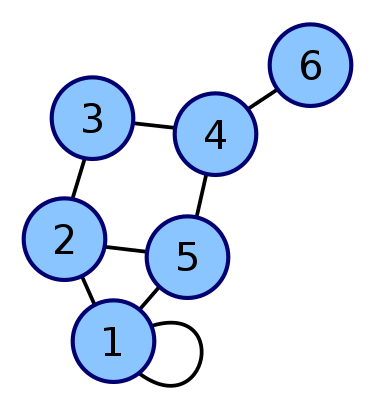
\includegraphics[height=8em]{images/3_graf-matice-souslednosti}

\caption[Ilustrační graf]{Ilustrační graf\\{\small (Chris-martin, Wikimedia Commons, volné dílo)}}
\label{ilustracni-graf-matice}
\end{figure}

\subsection{Handshaking lemma}

Handshaking lemmma je tvrzení že pro~každý konečný neorientovaný graf platí, že počet vrcholů s~lichým stupněm je sudý (formálně $\sum_{v \in V} \deg v = 2 |E|$: součet stupňů vrcholů odpovídá dvojnásobku počtu hran).

V~roce 1736 byla dokázána Leonardem Eulerem v~dokumentu řešícím problém \href{https://cs.wikipedia.org/wiki/Sedm_most%C5%AF_m%C4%9Bsta_Kr%C3%A1lovce}{Sedmi mostů města Královce}.
Graf obsahuje Eulerovskou cestu právě tehdy, když jím lze projít tak aby byla každá hrana navštívena právě jednou.

\subsection{Detekce bipartitního grafu}

Graf $G$ je bipartitní právě když je možné jeho vrcholy rozdělit do~dvou množin $V_1$ a~$V_2$ tak že každá hrana spojuje vrchol $V_1$ s~$V_2$.
Bipartitní grafy s~velikostí $|V_1|=m$ a~$|V_2|=n$ se značí $K_\mathrm{m,n}$.

Pro~detekci se využívá BFS:

\begin{enumerate}
\item Vyber bod grafu.
\item Přiřaď mu barvu a~označte ho za~navštívený.
\item Pokud má alespoň jeden sousední bod stejnou barvu jako aktuální bod, graf nelze obarvit dvěma barvami.
\item Všem sousedům přiřaď druhou barvu.
\item Přejdi do~některého ze sousedů který ještě nebyl navštívený.
\item Pokračuj dokud nejsou všechny body grafu obarvené.
\end{enumerate}

\subsection{Silně propojené komponenty}

\emph{Graf} je silně propojený tehdy, když je každý vrchol dosažitelný z~každého jiného vrcholu.
Silně propojené komponenty jsou podgrafy, které jsou samy o~sobě pevně propojeny.

\subsubsection{Kosarajův algoritmus}

Algoritmus hledající silně propojené komponenty pracující v~lineárním čase.
% TODO Tato poznámka je sice pravdivá, ale není zřejmá z pseudokódu
% Využívá faktu, že transponovaný graf $G^T$ má stejné silně propojené komponenty jako původní graf $G$.

\begin{figure}[ht]
\onehalfspacing
\begin{enumerate}
\item Označ každý vrchol grafu za~nenavštívený
\item Vytvoř zásobník L
\item Pro každý vrchol grafu V spusť podprogram Navštiv(V):
    \begin{itemize}
    \item Pokud je U nenavštívený:
        \begin{enumerate}
        \item Označ U jako navštívený
        \item Pro každého souseda N zavolej Navštiv(N)
        \item Přidej U na~vrchol zásobníku
        \end{enumerate}
    \item Jinak nedělej nic
    \end{itemize}
\item Pro každý vrchol V zásobníku L spusť podprogram Přiřaď(V,V):
    \begin{itemize}
    \item Pokud V nepatří žádné komponentě:
        \begin{enumerate}
        \item Přiřaď V komponentě A
        \item Pro každého souseda N zavolej Přiřaď(N,V)
        \end{enumerate}
    \item Jinak nedělej nic
    \end{itemize}
\end{enumerate}
\end{figure}
\FloatBarrier

\subsubsection{Tarjanův algoritmus}

Algoritmus hledající silně propojené komponenty pracující v~lineárním čase, efektivnější než Kosarajův.

\begin{figure}[ht]
\onehalfspacing
\begin{enumerate}
\item Označ každý vrchol grafu za~nenavštívený
\item Vytvoř zásobník
\item Vytvoř čítač \emph{i} a nastav ho na~0
\item Vyber nenavštívený vrchol \emph{v} a spusť nad ním podprogram Propoj(\emph{v}):
    \begin{enumerate}
    \item nastav \emph{v.index} a \emph{v.lowlink} na~\emph{i}
    \item zvyš čítač \emph{i} o 1
    \item přidej vrchol \emph{v} do~zásobníku
    \item pro každého navštívitelného souseda \emph{n}:
        \begin{itemize}
        \item pokud \emph{n} nebyl navštíven, nastav \emph{v.lowlink} na~\emph{min(v.lowlink, n.lowlink)}
        \item pokud je \emph{n} v~zásobníku, nastav \emph{v.lowlink} na~\emph{min(v.lowlink, n.index)}
        \end{itemize}
    \item pokud je \emph{v.lowlink} rovný \emph{v.index}:
        \begin{enumerate}
        \item vytvoř propojenou komponentu ze zásobníku
        \item vymaž zásobník
        \end{enumerate}
    \end{enumerate}
\end{enumerate}
\end{figure}
\FloatBarrier

\begin{figure}[ht]
\centering
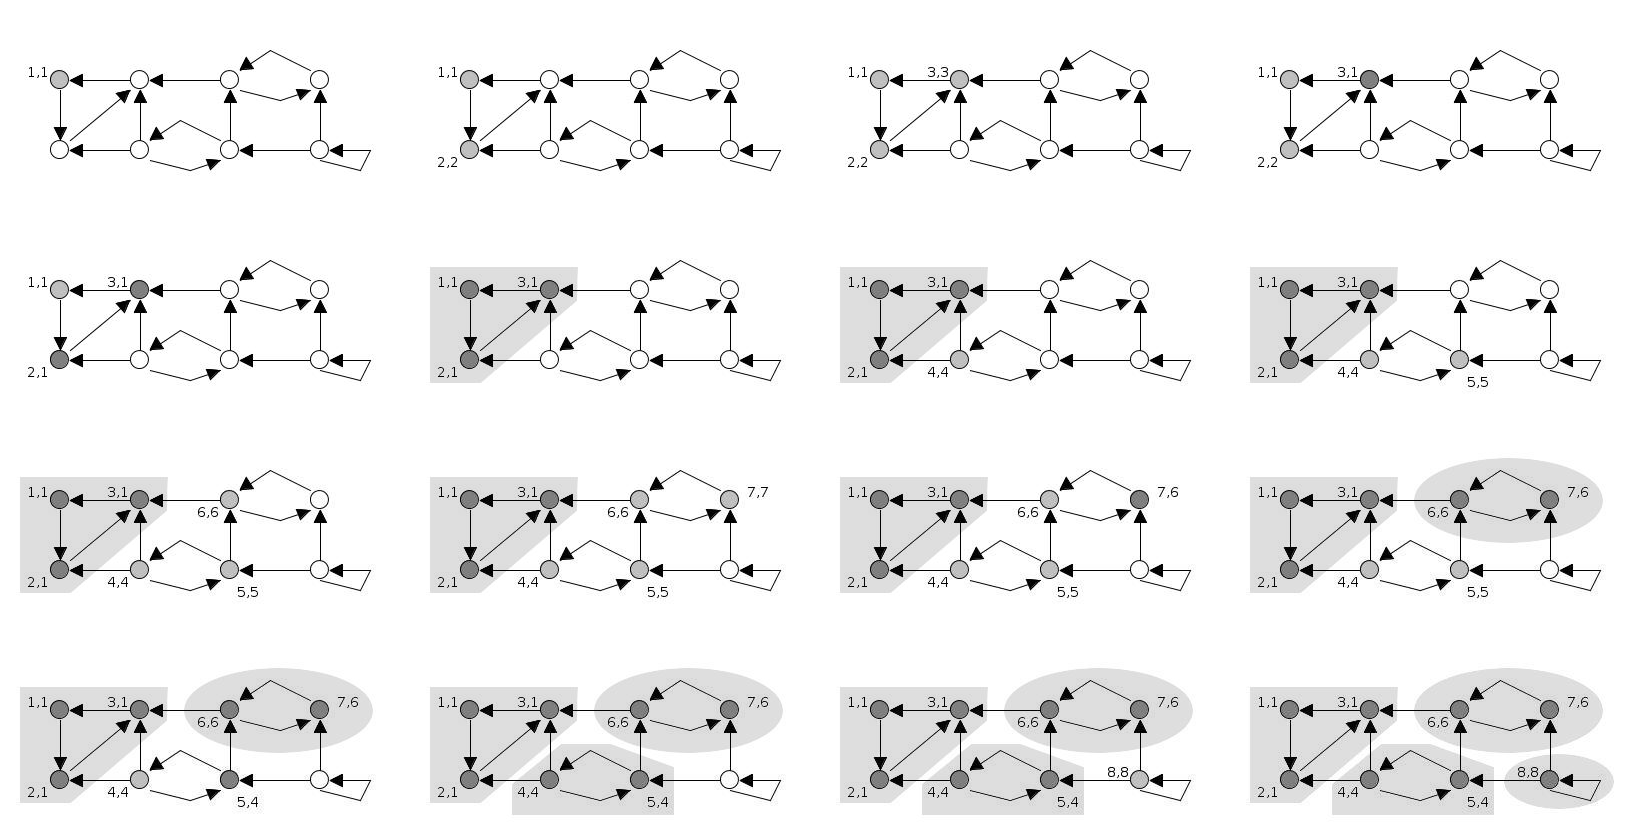
\includegraphics[width=\textwidth]{images/3_tarjanuv-algoritmus-animace.png}

\caption[Animace Tarjanova algoritmu]{Animace Tarjanova algoritmu\\{\small (LynX, Wikimedia Commons, CC BY-SA 3.0)}}
\end{figure}

\clearpage
\section{Vlastnosti grafu: průměr, excentricita. Párování grafu. Maďarský algoritmus. Problém časové tabule. Algoritmus barvení grafu. Izomorfismus grafu a Ullmanův algoritmus.}

Excentricita vrcholu $x$ grafu $G$ je maximální vzdálenost bodu od~jakéhokoliv bodu v~grafu: $\mathrm{e}(x) = \max\{ d_G(x, y) \ |\ y \in V_G\}$, kde $d_G(x,y)$ je minimální vzdálenost mezi body $x, y$.

{}Pro~poloměr grafu platí $\mathrm{r}(G) = \min\{ \mathrm{e}(x)\ |\ x \in V \}$.
\\Pro~průměr grafu platí $\mathrm{d}(G) = \max\{ \mathrm{e}(x)\ |\ x \in V \}$.

\subsection{Párování grafu}

Párování grafu je taková podmnožina hran grafu $M \subseteq E$, ve~které žádné dvě hrany nemají společný vrchol.
Vrcholy, které patří do~párování, se nazývají \emph{saturované}.

{}\emph{Maximální} párování má nejvíce hran (protože graf může mít párování více).
\\\emph{Perfektní} párování pokrývá všechny vrcholy grafu.

\subsubsection{Maďarský algoritmus}

Vstupem je matice $m \times n$ (řádky odpovídají \enquote{pracovníkům} a~sloupce \enquote{úkolům}).

\begin{enumerate}
    \item Všem polím v~každém řádku odečtěte nejnižší hodnotu řádku.
    \item Všem polím v~každém sloupci odečtěte nejnizší hodnotu sloupce.
    \item Nakreslete čáru přes řádky/sloupce tak aby překrývaly všechny nuly s~co nejmenším počtem čar (= pokrytí).
    \item Pokud je počet čar roven počtu řádků, algoritmus končí.
    \item Najděte nejmenší nepokrytou hodnotu. Odečtěte její hodnotu od~každého odkrytého řádku a~přidejte ji ke~každé nenulové hodnotě v~zakrytému sloupci. Vraťte se na~krok~3.
\end{enumerate}

Výsledkem je nějaká z~kombinací nenulových polí.

\subsection{Problém časového rozvrhu}

Ve~škole je $m$ učitelů a~$n$ tříd.
Učitel $i$ musí učit v~třídě $j$ v~semestru $P_{i,j}$.
Problémem je nalezení nejlepšího řešení.

Existuje mnoho verzí tohoto problému:
limitovaný počet učeben,
učitelé mohou učit jen v~určité časy,
žáci musí mít obědovou pauzu,
v~rozvrhu by neměly být zbytečné díry,
\dots

\subsubsection{Barvení grafů}

\paragraph{Largest Degree Ordering}

Vrcholy grafu jsou seřazeny sestupně dle jejich stupně.
Prochází se jimi postupně: vrchol je obarven takovou nejdřívější barvou, která se nevyskytuje u~jeho sousedů.

\paragraph{Incidence Degree Ordering}

Je vybrán vrchol s~nejvyšším stupněm, kterému je přiřazena první barva.
Pro~neobarvené vrcholy je spočítán počet obarvených sousedů a k~obarvení je vybrán ten s~jejich největším počtem.

\subsection{Izomorfismus grafů}

Grafy $G$ a $H$ jsou izomorfní, pokud mezi nimi existuje (hrany zachovávající) bijekce (mapování).

\subsubsection{Ullmanův algoritmus}

\clearpage
\section{Problém maximálního toku a~minimálního řezu grafem. Řešení problému s~více zdroji a~více cíli. Ford Fulkersonův algoritmus. Definice úzkého hrdla. Definice reziduální cesty.}

\subsection{Maximální tok grafem}

Maximální tok a~minimální řez jsou dva výrazy popisující stejný problém, pouze na~něj nahlíží z~jiných stran.

Pracuje se s~orientovaným váženým grafem $G$ se zdrojem $s$ a~cílem $t$, kde pro~každou hranu $e$ platí $c(e) \geq 0$ (kde $c$ je kapacita hrany).

Celkový tok na~vstupu se musí rovnat toku na~výstupu, každý nezdrojový a~neterminální bod musí mít shodnou kapacitu na~vstupu a~výstupu.

Pokud je vstupních/terminálních bodů více, nejsnažší řešení je jejich sloučení do~virtuálního uzlu s~nekonečnou kapacitou.

\subsubsection{Ford--Fulkersonova metoda}

\begin{figure}[ht]
\onehalfspacing
\begin{enumerate}
\item Začni s nulovým tokem
\item Dokud existují rozšiřující cesty:
    \begin{enumerate}
    \item Najdi rozšiřující cestu pomocí BFS
    \item Vypočítej úzké hrdlo pro danou cestu
    \item Pro~každý vrchol $u \rightarrow v$ na cestě
        \begin{enumerate}
        \item Zvyš tok $u \rightarrow v$ o~hodnotu hrdla
        \item Sniž tok $v \rightarrow u$ o~hodnotu hrdla
        \end{enumerate}
    \item Zvyš maximální tok o~hodnotu hrdla
    \end{enumerate}
\end{enumerate}
\end{figure}

FFM není plně specifikována; když se hovoří o~algoritmu, nazývá se Edmonds--Karpovým algoritmem.

\begin{figure}[ht]
\centering
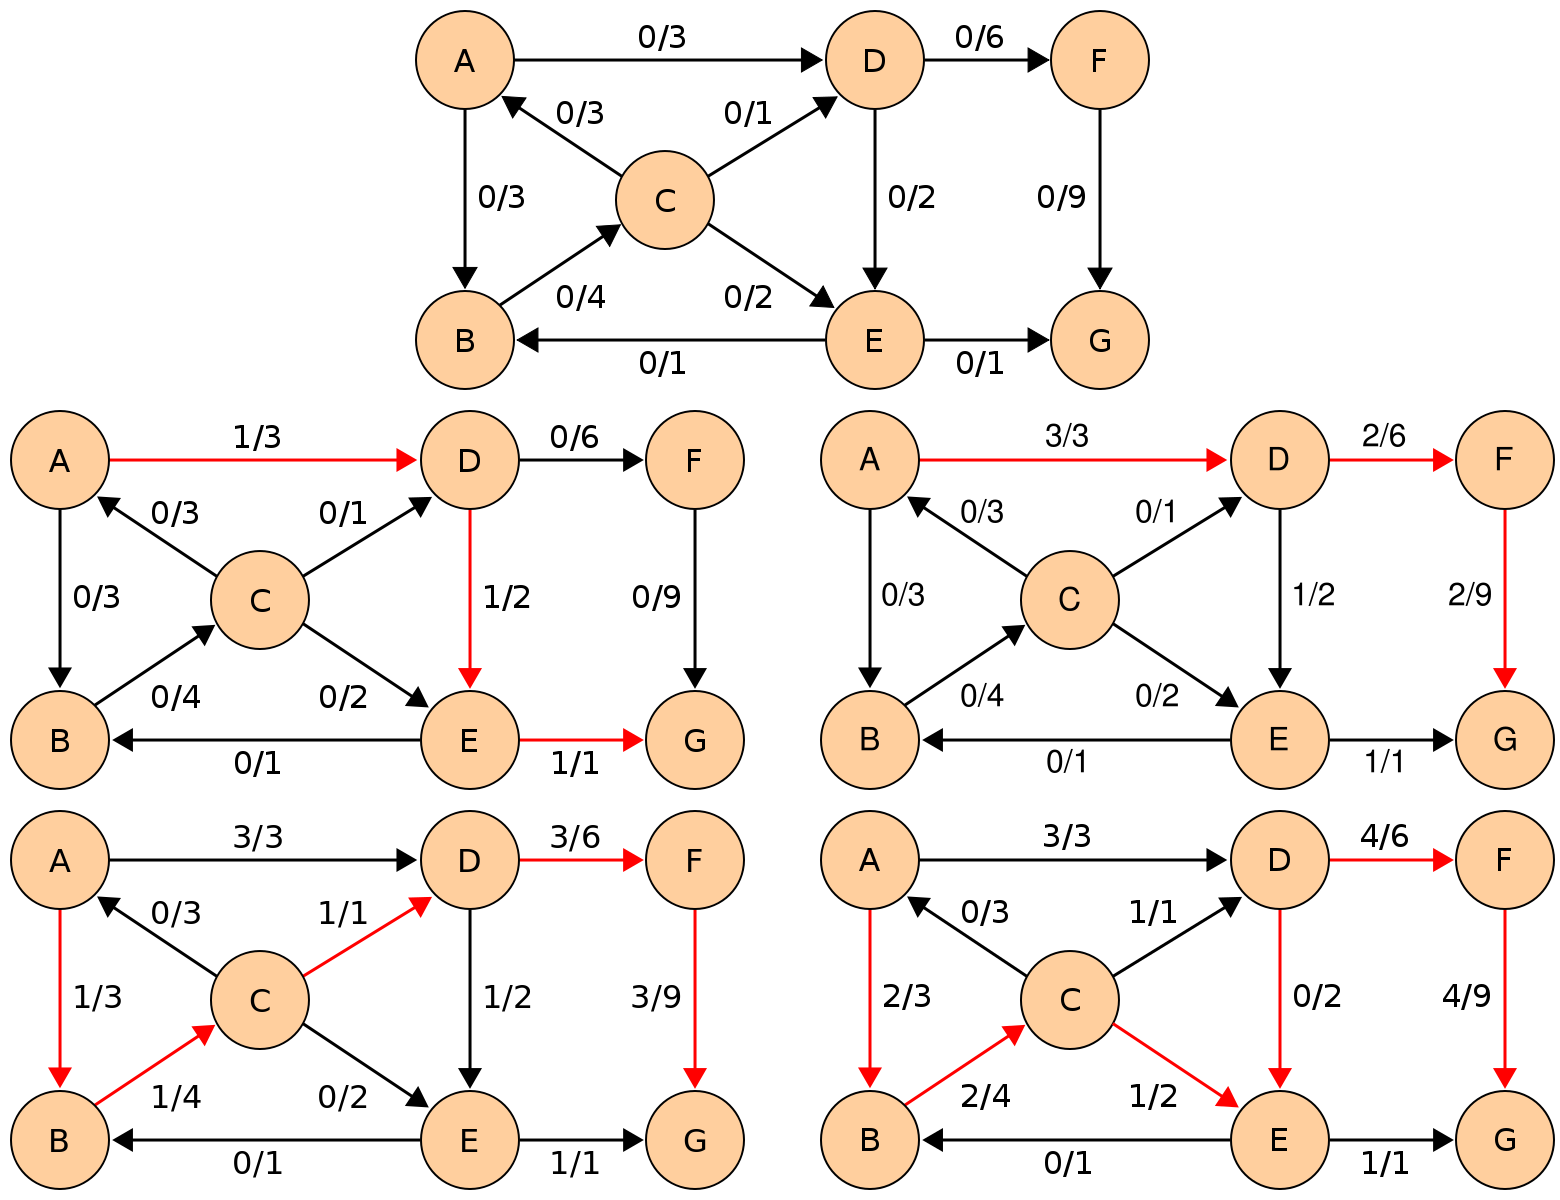
\includegraphics[width=\textwidth]{images/5_edmonds-karp}
\caption[Řešení maximálního proudu Edmonds--Karpovým algoritmem]{Řešení maximálního proudu Edmonds--Karpovým algoritmem\\{\small (Cburnett, Wikimedia Commons, CC BY-SA 3.0)}}
\end{figure}
\FloatBarrier

\subsection{Úzké hrdlo}

% TODO Nutno ověřit.
Úzké hrdlo cesty je minimální hodnota kapacity hrany na~této cestě.

Úzké hrdlo mezi dvěma vrcholy je maximum z~úzkých hrdel přes všechny cesty mezi těmito vrcholy.

Úzké hrdlo grafu je minimum z~úzkých hrdel cest mezi vstupem a~terminálem.

\subsection{Reziduální cesta}

Reziduální kapacita hrany je rozdíl kapacity a~proudu: $c_\mathrm{res}(u,v) = c(u,v) - f(u,v)$.

Reziduální cesta je cesta od~terminálu ke~vstupu vytvořená reziduálními hranami.

\clearpage
\section{Univerzální aproximační funkce. Dopředná neuronová síť. Maticová reprezentace NN. Gradientní sestup. Vrstva zahazování. Aktivační funkce. Softmax.}


\clearpage
\section{Konvoluční neuronové sítě – princip. Max pooling, Dávková normalizace. Známé architektury neuronových sítí.}


\clearpage
\section{Lineární regrese. Polynomiální regrese. Logistická regrese.}


\clearpage
\section{Rekurentní neuronové sítě. LSTM. UNet sítě. Struktury neuronových sítí.}


\clearpage
\section{Q-učení, srovnání s~genetickými algoritmy.}

\subsection{Zpětnovazební učení}

Zpětnovazební učení funguje na principu maximalizování výsledku bez toho aniž by věděl jak správně dosáhnout výsledku.
Zpětnovazební učení využívá algoritmů jako je Q-učení, SARSA, TD-učení a další.

\subsubsection{Rozdíl oproti genetickým algoritmům}

Hlavním rozdílem je, že zpětnovazební učení se snaží dosáhnout co nejlepšího výsledku, zatím co GA hledá spíše optimální výsledek.
Dalším rozdílem je, že GA výsledek měří dle fittnes zatímco zpětnovazební učení dle odměny (reward).

\subsection{Markov Decision Process (MDP)}

MDP se skládá ze čtyř částí a jedné volitelné:
\begin{itemize}
	\item $S$ je množina stavů (nejméně začátek a konec)
	\item $A$ je množina akcí (jaké akce lze provést)
	\item Transition state udává pravděpodobnost s~jakou skončím v~dalším stavu pokud jsem ve stavu $s$~a~provedu akci z~$A$. 
	\item Reward je odměna a~počítá se stejně jako Transition state jen výsledkem není pravděpodobnost, ale odměna, může být kladá nebo záporná
	\item $\gamma$ discount factor, je mezi $0 \leq \gamma \leq 1$ a ve výchozím stavu je 1 (volitelná)
\end{itemize}

\begin{figure}[h]
    \centering
	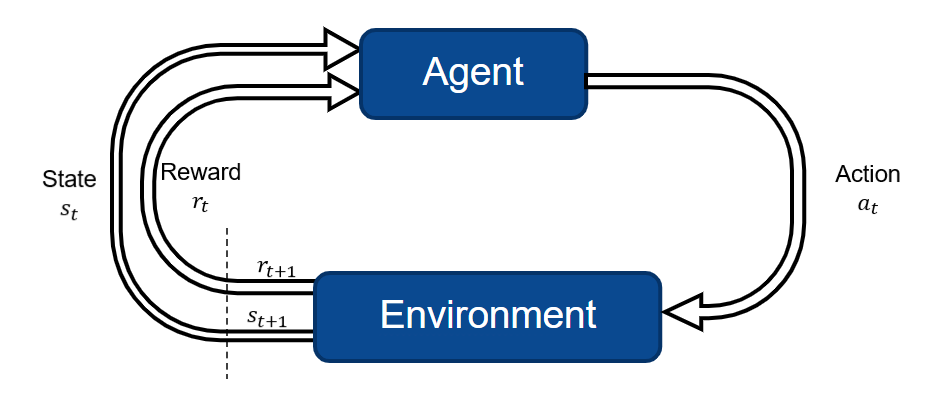
\includegraphics[height=10em]{images/10_MDP.png}
    \caption{Princip MDP}
    \label{mdp}
\end{figure}

\subsection{Q-učení}

V~Q-učení počet možných akcí a~stavů je konečný.
Je založeno na MDP.

Výběr akce v~závislosti na aktuálním stavu se vybírá dle Q-value.
Q-value určuje vhodnost (kvalitu) akce v~daném stavu.
Q-value se vypočítají jako odhad dalších odměn ve zbylých krocích aktuálního příběhu.
Příběh nebo epizoda je jedna iterace učení, jakoby pokus.
Takže čím blíže jsme k~cíli tím víc narůstá Q-value.

Q-value pro každý stav a~akci se zapíše do Q-table. 

\subsubsection{Exploration vs exploitation}

Exploration slouží pro prozkoumání prostředí a~nalezení informací o~něm.

Exploitation slouží k~využítí znalosí o~prostředí.

Ve zpětnovazebním učení se musí docílít optimalizace mezi exploration a~exploitation.
K~této optimalizaci se využívá epsilon greedy strategy.
Epsilon greedy strategy využívá hodnoty $\epsilon$, která slouží k~určení poměru při rozhodování.
V~počátečních příbězích je nastaveno $\epsilon$ na 1 což značí, že se bude probíhat pouze exploration. 
V~dalších příbězích se $\epsilon$ pomalu snižuje.

\subsubsection{Aktualizace Q-value}

Probíhá dle rovnice:

$q^\text{new}(s,a) = (1-\alpha)q(s,a) + \alpha \left(R_{t+1} + \gamma\,\text{max}\,q(s',a')\right)$

Hodnota $\alpha$ je learning rate, který určuje kolik informací z~přechozí Q-value chceme ponechat.
Nabývá hodnot 0 až 1 ($0\leq\alpha\leq1$).
Čím vyšší je tato hodnota tím rychleji se projeví nová hodnota Q-value. 

Hodnota $q(s,a)$ určuje předchozí Q-value.

Hodnota $\left(R_{t+1} + \gamma\,\text{max}\,q(s',a')\right)$ určuje momentální (novou) vypočítanou Q-value.

Takže aktualizovaná Q-value je stará hodnota + nová.


\subsubsection{Jak v krocích funguje Q-learning}

\begin{enumerate}
    \item Inicializace Q-values v~Q-table
    \item Pro každý příběh
    \begin{enumerate}
    	\item Výběr mezi exploration a~exploitation (náhodná generace čísla)
    	\item Provede se akce
    	\item Aktualizuje se Q-value 
    \end{enumerate}
    \item Po ukončení příběhů je připravená Q-table
\end{enumerate}

\subsection{Q-učení vs SARSA}

Sarsa používá politiku (policy) chovaní k výběru další akce.
Q-učení nevyužívá politiku k~výběru další akce, ale odhaduje budoucí výnosu, které aktualizuje.



\clearpage
\section{Extrakce znalostí ze stromových a grafových struktur. Metoda náhodného průchodu. Node2Vec. Obecná umělá inteligence – relační induktivní zaměření, kombinatorická generalizace. Předávání zpráv.}

Klasicky jsou data pro strojové učení uspořádana ve vektoru (1D, 2D). 
Využívá se k~tomu nejčastěji lineární regrese nebo CNN (konvoluční neuronové sítě). 
Pokud bychom chtěli převést stromovou nebo grafovou strukturu do~vektrou, bude to možné aproximací, a~dojde ke~ztrátě některých informací.
Proto se využívá různých metod na~převedení grafové struktury na~zpracovatelné podoby pomocí embedding nodes.

\subsection{Embeddings nodes}

Využívá DeepWalk metodu (první metoda). 
Ukazuje jak by vypadal graf ve~2D, kdy podobné vrcholy jsou v~tomto prostoru blízko při sobě.

\begin{figure}[ht]
    \centering
    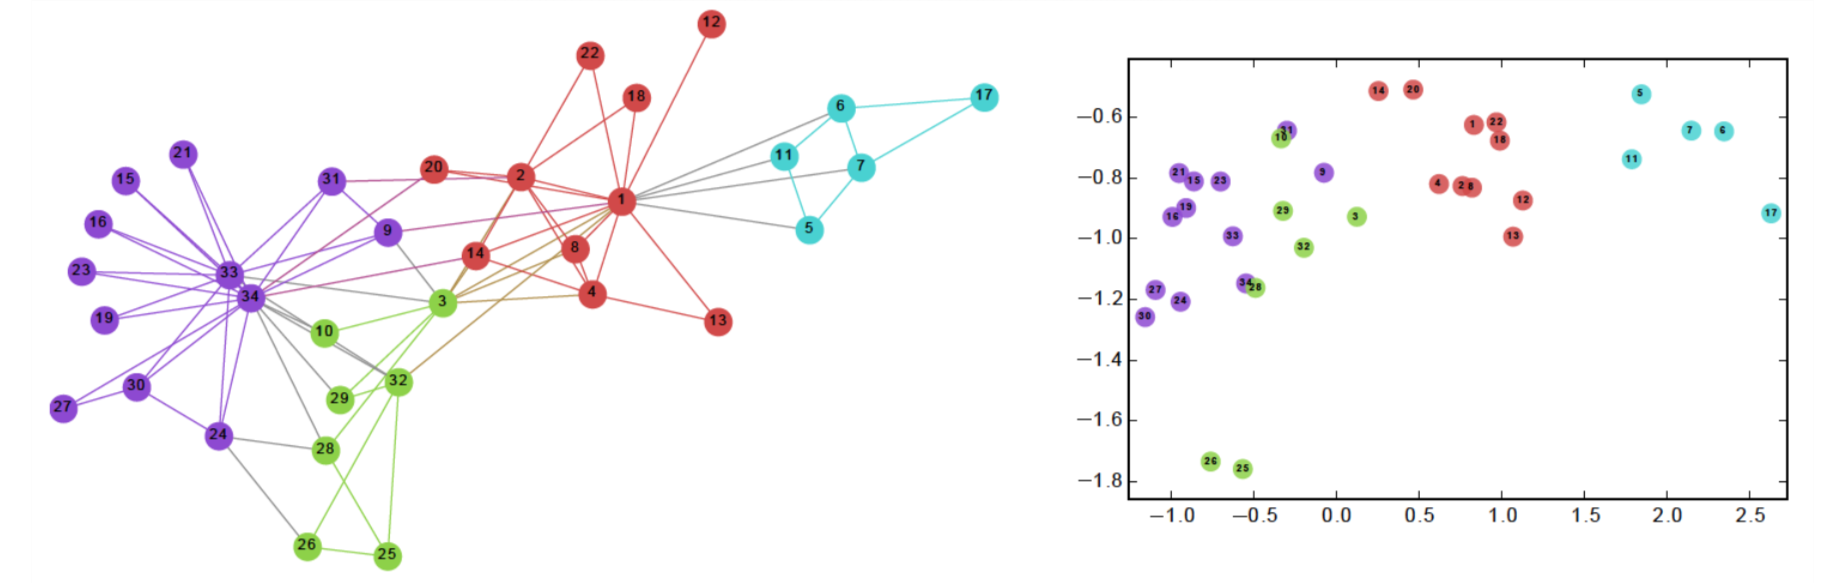
\includegraphics[width=\textwidth]{images/11_deepwalk-graf}
    \caption{DeepWalk metoda}
\end{figure}

Cílem je zakódovat vrcholy z~grafu do~embedding prostoru tak že podobnost v~embedding prostoru se blíží podobnosti grafu.
Tento cíl udává rovnice:
$\text{similarity}(u,v)\approx \mathbf{z}_{v}^{T}\,\mathbf{z}_{u}$

Máme encoder, který mapuje vrcholy na~embeddings. 
Poté je fuknce na~výpočet podobnosti (v~rovnici levá strana), která měří podobnost v~originálním grafu (síti).
Následně je decoder (pravá strana rovnice), který mapuje embeddings na~hodnotu podobnosti (similarity score).
Nakonec se parametry encoderu optimalizují tak aby platila rovnice.

\begin{figure}[ht]
    \centering
    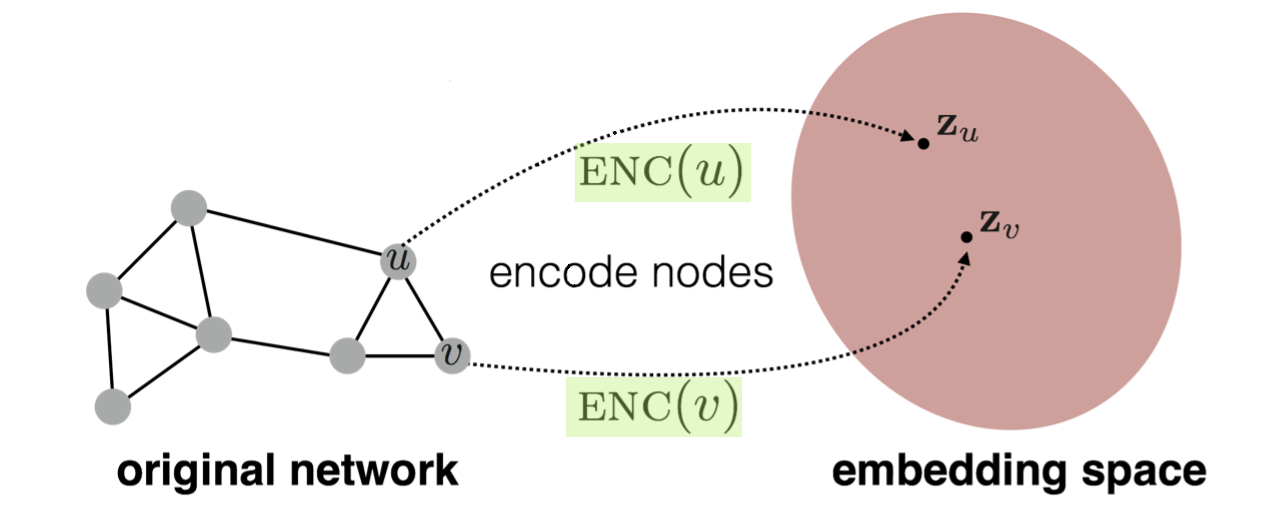
\includegraphics[height=10em]{images/11_similarity}
    \caption{Podobnost mezi grafem a embedding prostorem}
\end{figure}

\subsection{random-walk embedding}

Pravděpodobnost, že $u$ a $v$ se společně vyskytnou na~náhodné cestě grafem je rovna nebo přibližná $\mathbf{z}_{v}^{T}\,\mathbf{z}_{u}$.

\subsubsection{Přoč random-walk}

{}Expressivity: podobnost vrcholů zahrnujících místní i~high-order neighborhood informace.
\\Efficiency: musí se uvažovat pouze páry vrcholů, které se společně vyskytují na~random-walk cestě.

\subsubsection{Postup}

Nejprve se odhadne pravděpodobnost navštívení vrcholu $v$ na~náhodné cestě grafem začínající v~bodě $u$, využívající některou random-walk strategii. 
Následně se optimalizuje embeddings k~zakódování random-walk statistik.

\subsubsection{Optimalizace postup}

Nejprve se spustí random-walk s~krátkou pevnou délkou, který startuje z~každého vrcholu $u$ v~grafu využívající nějakou random-walk strategii.
Dále pro každý vrchol $u$ se sesbírá množina navštívených vrcholů pomocí na~cestě (pomocí random-walk strategie) začínajících z~$u$.
Nakonec se optimalizuje embeddings (pro vrchol $u$ dokážeme předpovědět sousedy v~množině).

$$\mathcal{L} = \sum_{u\in V} \sum_{v\in N_R (u)} - \log(\frac{\exp(\mathbf{z}_{u}\,\mathbf{z}_{v})}{\sum_{n\in V} \exp(\mathbf{z}_{u}\,\mathbf{z}_{n})})$$

První suma značí součet přes všechny vrcholy $u$.
Druhá suma značí součt přes vrcholy $v$ vyskytujících se na~cestě z~vrcholu $u$.
Obsah logaritmu značí předpovídanou pravděpodobnost společného výskytu $u$ a $v$ na~cestě.

Cílem je najít $z_u$ které minimalizuje $\mathcal{L}$.


\subsubsection{node2vec}

Node2vec je velice podobný Deepwalk s~tím rozdílem, že jsou jinak vybírany sousední vrcholy.
Hlavní myšlenkou je kompromis mezi lokálním (BFS) a globálním (DFS) pohledem na~graf (síť).
Node2vec má dva parametry:
\begin{itemize}
	\item $p$ udávajací hodnotu návratu k~předchozímu vrcholu (return parameter)
	\item $q$ udavající \enquote{poměr} mězi BFS a DFS (\enquote{walk away} parameter)
\end{itemize}

Při zvolení $q>p$ se algoritmus zaměřuje spíše na~globální pohled (bude směřovat k~DFS průchodu). Při zvolení $q<p$ se algoritmus zaměří spíše na~lokalní pohled (bude směřovat k~BFS).

\begin{figure}[ht]
    \centering
	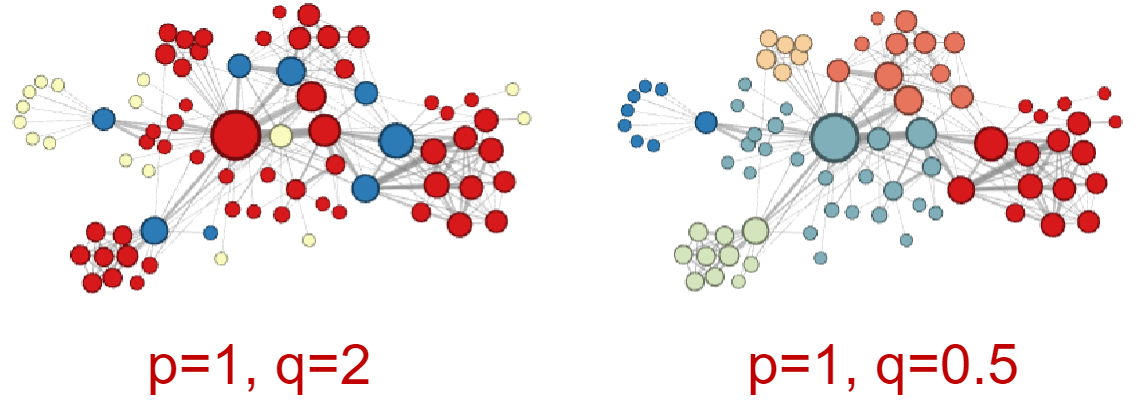
\includegraphics[width=\textwidth]{images/11_node2vec-pq}
    \caption{Prioritizace $p$ nebo $q$ v~node2vec}
\end{figure}

Při prochocházení grafem (viz obr.~\ref{pruchod-node2vec}) může dojít ke třem stavům (z~hlediska bodu $w$):
\begin{itemize}
	\item návrat k~předchozímu vrcholu ($s1$),
	\item navštívení vedlejšího vrcholu, který má stejnou vzdálenost od~počátečního vrcholu ($s2$)
	\item navštívení vzdálenějšího vrcholu ($s3$)
\end{itemize}

\begin{figure}
    \centering
	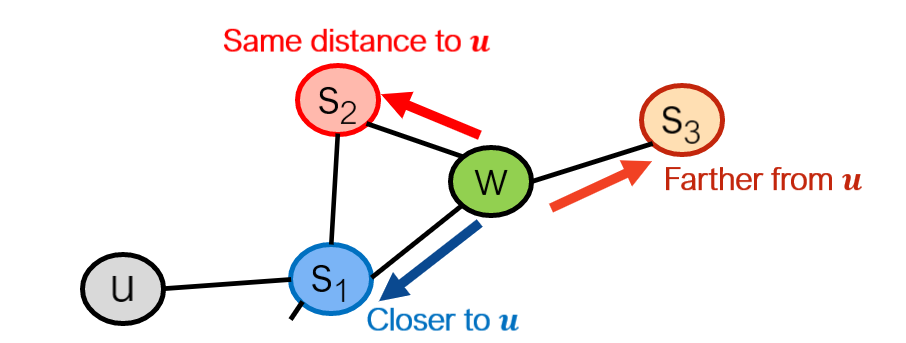
\includegraphics[height=10em]{images/node2vec.png}
    \caption{Průchod grafem v~node2vec}
    \label{pruchod-node2vec}
\end{figure}

\subsection{Relační induktivní zaměření}

Definice: Jak algoritmus preferuje jeden model před druhým. 

Existuje několik modelů:
\begin{table}[ht]
\centering
\caption{Vlastnosti komponent}
\begin{tabular}{|l|c|c|}
\hline
Komponent & Entita & Vazba (relace) \\ \hline \hline
Plně propojené & Units & All-to-all \\ \hline
Konvoluční & Grid elements & Local \\ \hline
Rekurentní & Timesteps & Sequential \\ \hline
Graph network & Vrchol & Hrana \\ \hline
\end{tabular}
\end{table}

\begin{figure}[ht]
    \centering
	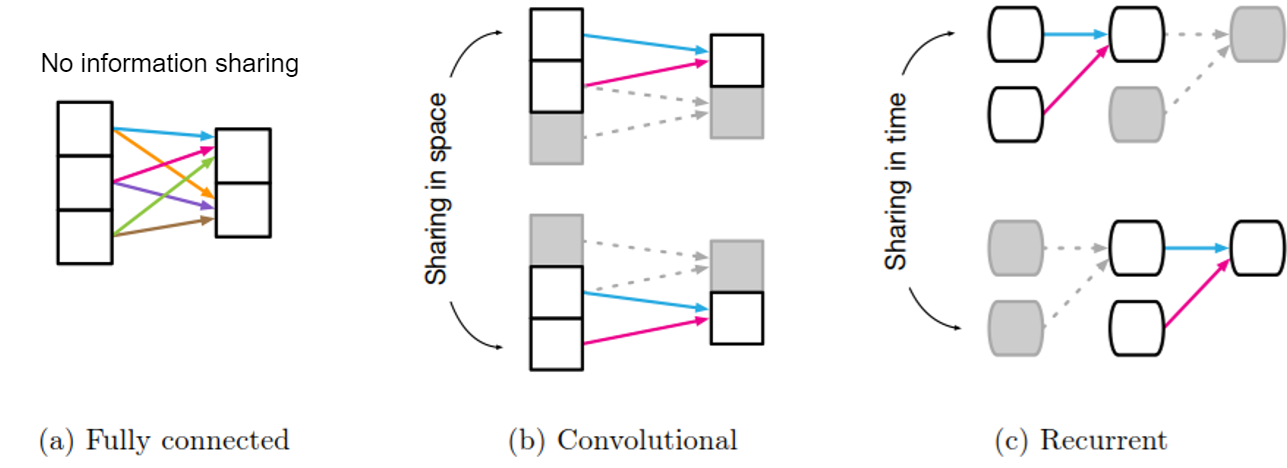
\includegraphics[width=\textwidth]{images/11_RIB}
    \caption{Přístupy relačního induktivního zaměření}
\end{figure}

\subsection{Kombinatirická generalizace}

Kombinatorická generalizace je vlastnost vytvářet nové rozhraní, predikce a chování z~už známých stavebních bloků.

Příkladem je vycestovat na~nové místo.
Máme známé postupy -- cestovat letadlem; do~Brna; dát si oběd; v~menze.
Generalizace je nalezení spojitostí mezi těmito věcmi na~už známých znalostech.

\subsection{Předávání zpráv}
\tikzstyle{vertexnocolor}=[circle, draw]

Mějme graf $G$ (viz obr.~\ref{graf-pro-predavani-zprav}) reprezentovatelný maticí souslednosti $\mathbf{A}$: 
$\left[ \begin{matrix}
0 & 1 & 0 & 0 & 0 \\
1 & 0 & 1 & 0 & 0 \\
0 & 1 & 0 & 1 & 1 \\
0 & 0 & 1 & 0 & 0 \\
0 & 0 & 1 & 0 & 0 \\
\end{matrix} \right]$.

\begin{figure}[ht]
    \centering
    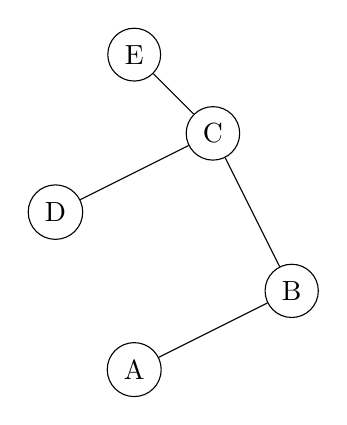
\begin{tikzpicture}
		\node[vertexnocolor](a) at (1, -2) {A};
        \node[vertexnocolor](b) at (3, -1) {B};
        \node[vertexnocolor](c) at (2, 1) {C};
        \node[vertexnocolor](d) at (0, 0) {D};
        \node[vertexnocolor](e) at (1, 2) {E};
            
        \begin{scope}[every path/.style={-}, every node/.style={inner sep=1pt}]
        	\draw (a) -- node [anchor=east] {} (b);
                   
            \draw (b) -- node [anchor=east] {} (c);
                   
            \draw (c) -- node [anchor=east] {} (d);
            \draw (c) -- node [anchor=east] {} (e);
		\end{scope}
	\end{tikzpicture}
    \caption{Graf $G$.}
    \label{graf-pro-predavani-zprav}
\end{figure}
\FloatBarrier

Po tomto bodu záleží jakou metodu zvolíme.

\subsubsection{Součet sousedních vrcholů}

Zvolíme matici $\mathbf{H_1}$, která bude reprezentovat hodnoty vrcholů:
$\left[ \begin{matrix}
1 \\
2 \\
3 \\
4 \\
5 \\
\end{matrix} \right]$.

Vynásobíme matici $\mathbf{A}$ maticí $\mathbf{H_1}$ a~získáme předávanou zprávu.

$$
\left[ \begin{matrix}
0 & 1 & 0 & 0 & 0 \\
1 & 0 & 1 & 0 & 0 \\
0 & 1 & 0 & 1 & 1 \\
0 & 0 & 1 & 0 & 0 \\
0 & 0 & 1 & 0 & 0 \\
\end{matrix} \right]
\left[ \begin{matrix}
1 \\
2 \\
3 \\
4 \\
5 \\
\end{matrix} \right] = 
\left[ \begin{matrix}
0 \cdot 1 + 1 \cdot 2 + 0 \cdot 3 + 0 \cdot 4 + 0 \cdot 5 \\
1 \cdot 1 + 0 \cdot 2 + 1 \cdot 3 + 0 \cdot 4 + 0 \cdot 5 \\
0 \cdot 1 + 1 \cdot 2 + 0 \cdot 3 + 1 \cdot 4 + 1 \cdot 5 \\
0 \cdot 1 + 0 \cdot 2 + 1 \cdot 3 + 0 \cdot 4 + 0 \cdot 5 \\
0 \cdot 1 + 0 \cdot 2 + 1 \cdot 3 + 0 \cdot 4 + 0 \cdot 5 \\
\end{matrix} \right] = 
\left[ \begin{matrix}
2 \\
4 \\
11 \\
3 \\
3 \\
\end{matrix} \right]
$$

\subsubsection{Průměr sousedních vrcholů}

Kromě matice sousednosti se vytvoří matice stupňů vrcholu $\mathbf{D}$:
$\left[ \begin{matrix}
1 & 0 & 0 & 0 & 0 \\
0 & 2 & 0 & 0 & 0 \\
0 & 0 & 3 & 0 & 0 \\
0 & 0 & 0 & 1 & 0 \\
0 & 0 & 0 & 0 & 1 \\
\end{matrix} \right]$

Matice $\mathbf{D}$ se invertuje ($\frac{1}{x}$) kde $x$ je hodnota z~matice:
$\left[ \begin{matrix}
1 & 0 & 0 & 0 & 0 \\
0 & 0.5 & 0 & 0 & 0 \\
0 & 0 & 0.33 & 0 & 0 \\
0 & 0 & 0 & 1 & 0 \\
0 & 0 & 0 & 0 & 1 \\
\end{matrix} \right]$

Invertovaná matice se vynásobí s~maticí sousednosti, kde vznikne matice $\mathbf{A_\mathrm{avg}}$.

$$
\left[ \begin{matrix}
1 & 0 & 0 & 0 & 0 \\
0 & 2 & 0 & 0 & 0 \\
0 & 0 & 3 & 0 & 0 \\
0 & 0 & 0 & 1 & 0 \\
0 & 0 & 0 & 0 & 1 \\
\end{matrix} \right]
\left[ \begin{matrix}
1 & 0 & 0 & 0 & 0 \\
0 & 0.5 & 0 & 0 & 0 \\
0 & 0 & 0.33 & 0 & 0 \\
0 & 0 & 0 & 1 & 0 \\
0 & 0 & 0 & 0 & 1 \\
\end{matrix} \right] =
\left[ \begin{matrix}
0 & 1 & 0 & 0 & 0 \\
0.5 & 0 & 0.5 & 0 & 0 \\
0 & 0.33 & 0 & 0.33 & 0.33 \\
0 & 0 & 1 & 0 & 0 \\
0 & 0 & 1 & 0 & 0 \\
\end{matrix} \right]
$$

Tato výsledná matice se vynásobí z~maticí $\mathbf{H_1}$ a získáme předávanou zprávu.

$$
\left[ \begin{matrix}
0 & 1 & 0 & 0 & 0 \\
0.5 & 0 & 0.5 & 0 & 0 \\
0 & 0.33 & 0 & 0.33 & 0.33 \\
0 & 0 & 1 & 0 & 0 \\
0 & 0 & 1 & 0 & 0 \\
\end{matrix} \right]
\left[ \begin{matrix}
1 \\
2 \\
3 \\
4 \\
5 \\
\end{matrix} \right] = 
\left[ \begin{matrix}
2 \\
2 \\
3.6 \\
3 \\
3 \\
\end{matrix} \right] 
$$

\subsubsection{Průměr sousedních vrcholů a sám sebe}

Do~matice sousednosti doplníme, že každý vrchol sousedí sám se sebou a získáme $\mathbf{\tilde{A}}$:
$\left[ \begin{matrix}
1 & 1 & 0 & 0 & 0 \\
1 & 1 & 1 & 0 & 0 \\
0 & 1 & 1 & 1 & 1 \\
0 & 0 & 1 & 1 & 0 \\
0 & 0 & 1 & 0 & 1 \\
\end{matrix} \right]$.

Výsledná přenášená zpráva se vypočítá pomocí vzorce
$\mathbf{\hat{A}} = \mathbf{D}^{-\frac{1}{2}}\mathbf{\tilde{A}}\mathbf{\tilde{D}}^{-\frac{1}{2}}$.
